\documentclass{article}

\usepackage{graphicx}
\usepackage{tikz}
\usepackage{tikzsymbols}
\usetikzlibrary{calc,patterns,shapes.geometric}
\pagestyle{empty}
\usepackage[margin=0pt]{geometry}
\geometry{papersize={14in,12in}}

\def\centerarc[#1](#2)(#3:#4:#5){\draw[#1] ($(#2)+({#5*cos(#3)},{#5*sin(#3)})$) arc (#3:#4:#5);}

\begin{document}
	\begin{figure}
		\centering
		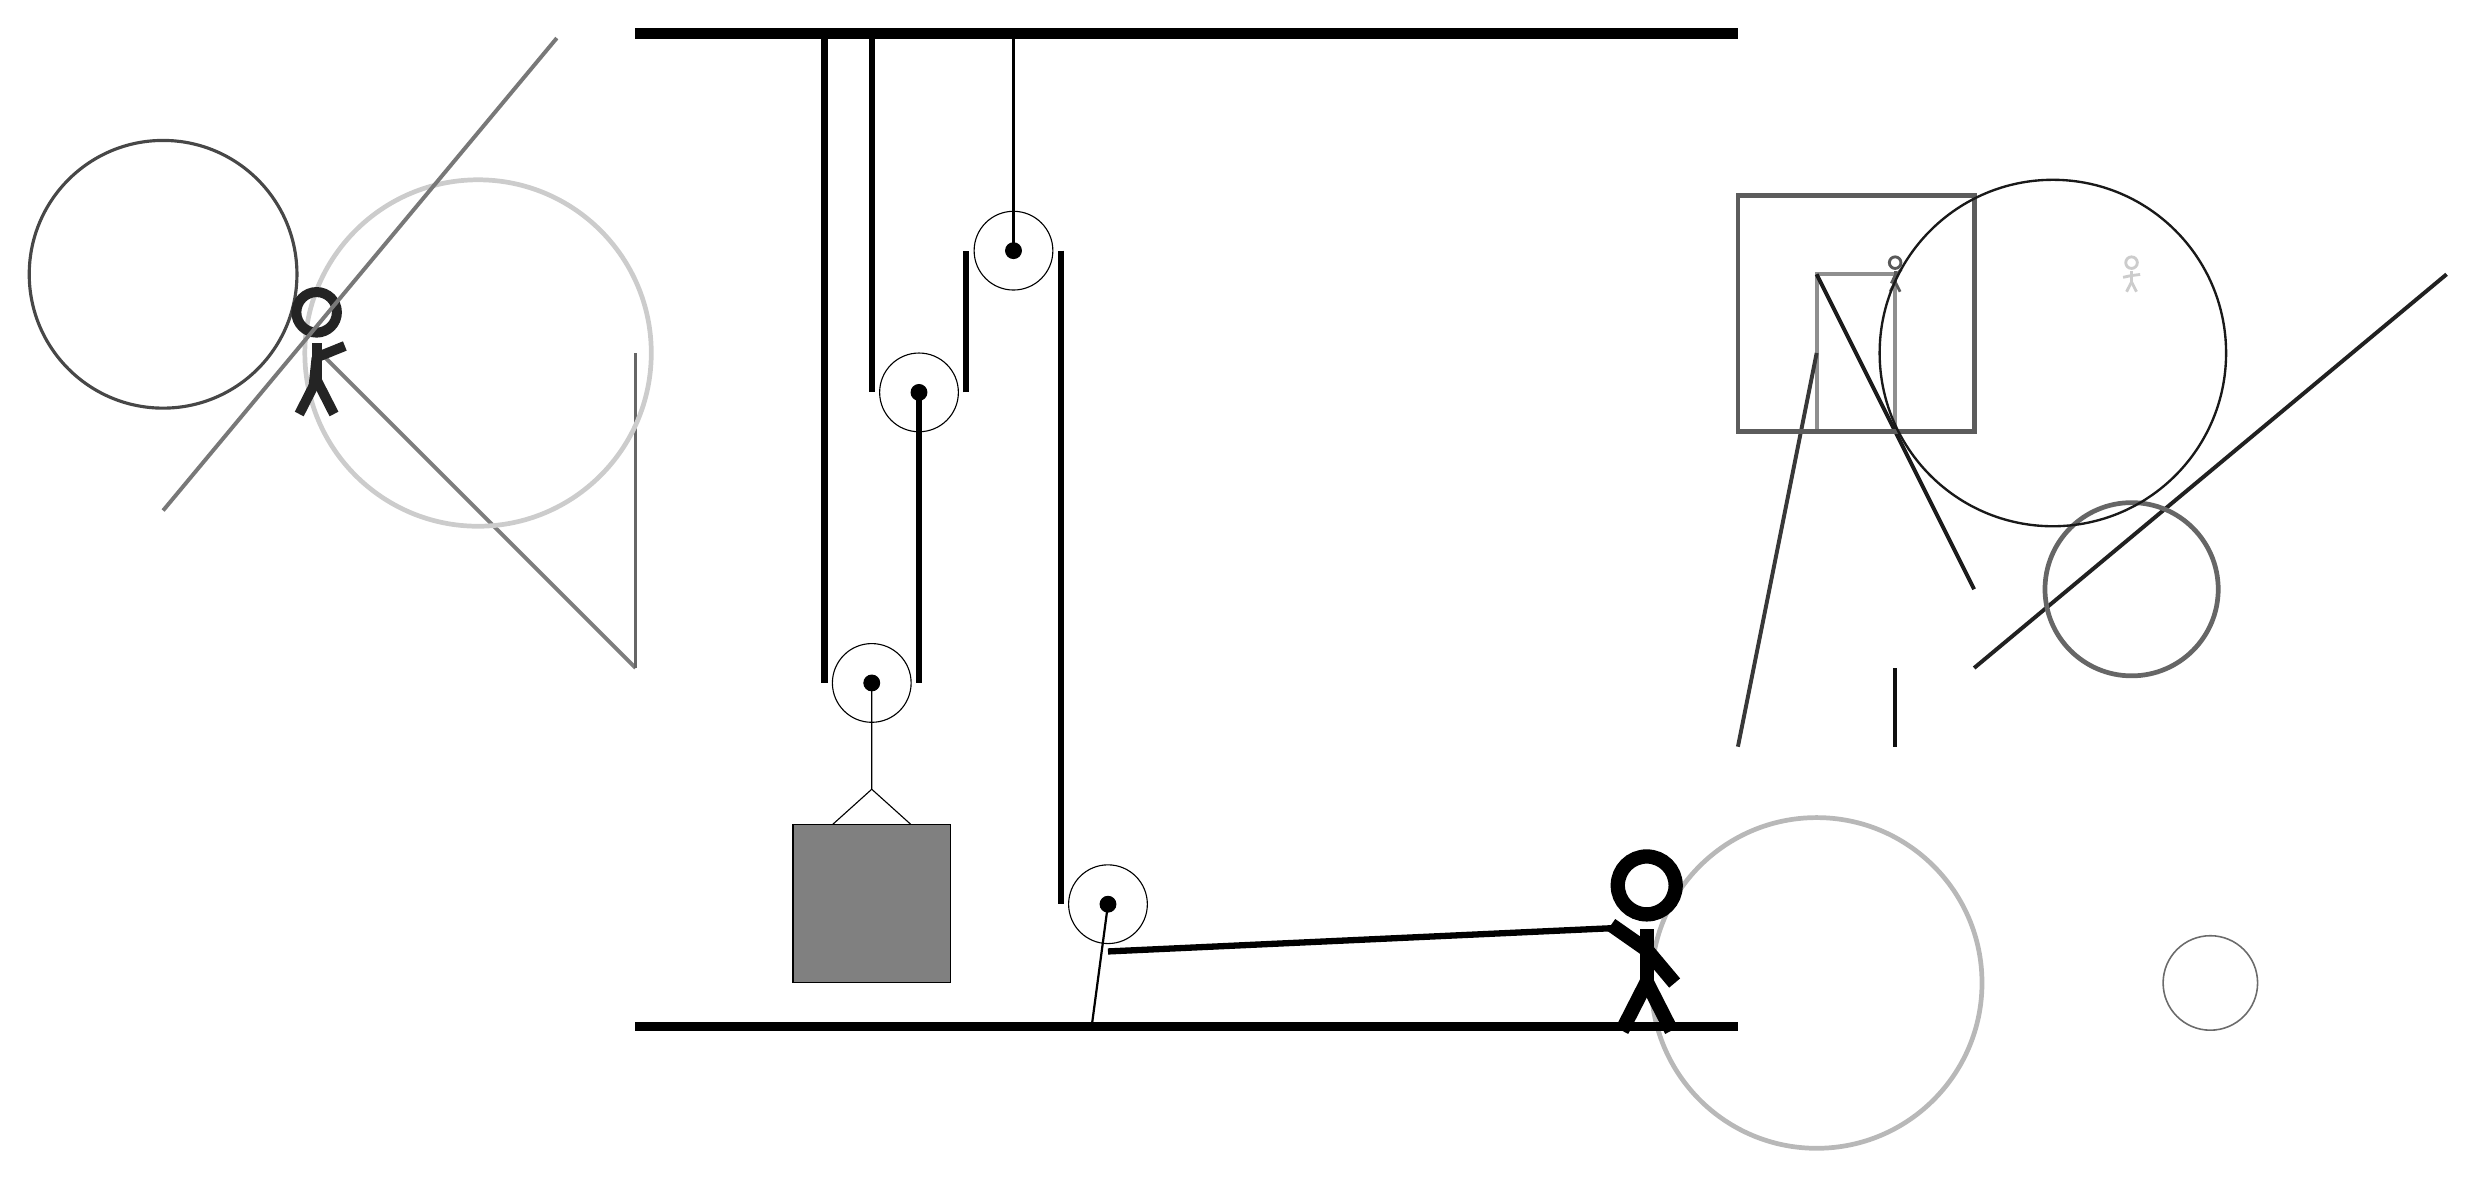
\begin{tikzpicture}
			%%%%% START %%%%%
			
			\draw[fill=black] (-2, 9) rectangle (12, 9.125);
			
			\draw (1, 0.81) circle (0.5);
			\draw[fill=black] (1, 0.81) circle (0.1);
			
			\draw[line width=0.5mm, color=black!51](-2, 1) -- (-6, 5);
			
			\draw [line width=0.4mm, color=black!72](-8, 6) circle (1.7);
			\draw[line width=0.5mm, color=black!44] (14, 4) rectangle (13, 6);
			\draw[line width=0.5mm, color=black!78](12, 0) -- (13, 5);
			\draw[line width=0.3mm, color=black!60] (-2, 1) rectangle (-2, 5);
			\draw[line width=0.5mm, color=black!87](15, 1) -- (21, 6);
			
			\draw [line width=0.2mm, color=black!58](18, -3) circle (0.6);
			\draw[line width=0.5mm, color=black!89](13, 6) -- (15, 2);
			\draw [line width=0.6mm, color=black!20](-4, 5) circle (2.2);
			\node[line width=0.5mm, color=black!86] at (-6, 5) {\Strichmaxerl[7][84][22]};
			\node[line width=0.6mm, color=black!65] at (14, 6) {\Strichmaxerl[2][64][44]};
			\draw [line width=0.6mm, color=black!28](13, -3) circle (2.1);
			\draw[line width=0.6mm, color=black!64] (12, 7) rectangle (15, 4);
			
			\draw [line width=0.6mm, color=black!60](17, 2) circle (1.1);
			\draw[line width=0.5mm, color=black!94](14, 0) -- (14, 1);
			\draw[line width=0.5mm, color=black!53](-3, 9) -- (-8, 3);
			\draw [line width=0.3mm, color=black!90](16, 5) circle (2.2);
			\node[line width=0.4mm, color=black!20] at (17, 6) {\Strichmaxerl[2][12][7]};
			
			\draw (1.6, 4.5) circle (0.5);
			\draw[fill=black] (1.6, 4.5) circle (0.1);
			
			\draw (2.8, 6.3) circle (0.5);
			\draw[fill=black] (2.8, 6.3) circle (0.1);
			\draw[thick] (2.8, 6.3) -- (2.8, 9);
			
			\draw (4.0, -2) circle (0.5);
			\draw[fill=black] (4.0, -2) circle (0.1);
			\draw[thick] (4.0, -2) -- (3.8, -3.5);
			
			\draw (1, 0.81) -- (1, -0.54) -- (0.5, -0.99) -- (1.5, -0.99) -- (1, -0.54);
			\draw[fill=black!50] (0, -0.99) rectangle (2, -2.99);
			\draw[line width=0.8mm] (0.4, 9) -- (0.4, 0.81);
			\centerarc[line width=0.8mm](1, 0.81)(180:360:0.6);
			\draw[line width=0.8mm](1.6, 0.81) -- (1.6, 4.5);
			\draw[line width=0.8mm] (1.0, 9) -- (1.0, 4.5);
			\centerarc[line width=0.8mm](1.6, 4.5)(180:360:0.6);
			\draw[line width=0.8mm](2.2, 4.5) -- (2.2, 6.3);
			\centerarc[line width=0.8mm](2.8, 6.3)(0:180:0.6);
			\draw[line width=0.8mm] (3.4, 6.3) -- (3.4, -2);
			\centerarc[line width=0.8mm](4.0, -2)(0:90:-0.6);
			\draw[line width=0.8mm](4.0, -2.6) -- (10.5, -2.3);
			
			\node at (10.8, -2.5) {\Strichmaxerl[10][-35][-50]};
			
			\draw[fill=black] (-2, -3.5) rectangle (12, -3.6);
			
			%%%%% END %%%%%
		\end{tikzpicture}
	\end{figure}	
\end{document}